\documentclass[11pt,pointlessnumbers,DIV10,BCOR10mm,tocleft]{scrreprt}
\setcounter{tocdepth}{2} 
%\typearea[5mm]{13}

% --- ALLGEMEINES; EINGABE; ZEICHEN ---
%\usepackage[T1]{fontenc}
\usepackage[utf8]{inputenc}
\usepackage[ngerman]{babel}
\usepackage{amssymb,amsmath,amsfonts,stmaryrd}
\usepackage{wasysym,relsize}

% --- INDEX ---
\usepackage{makeidx}
\makeindex

% --- DIVERSES ---
\usepackage{graphicx}
\usepackage{enumerate}


% --- FARBEN UND PSTRICKS ---
\usepackage{color,pstricks}
\newgray{gray}{0.25}
\newgray{komagray}{0.4}
\newgray{lightgray}{0.45}
\newgray{verylightgray}{0.65}
\newgray{verydarkgray}{0.15}
\newrgbcolor{green}{0 0.75 0}

% --- TITELFARBEN ---
\newrgbcolor{screenblue} {0.588 0.667 0.745}
\newrgbcolor{Screenblue} {0.275 0.431 0.667}
\newrgbcolor{dekoblue}   {0.392 0.588 0.863}
\newrgbcolor{screenbrown}{0.851 0.851 0.816}
\newrgbcolor{Screenbrown}{0.824 0.824 0.784}
\newrgbcolor{SCREENBROWN}{0.745 0.745 0.725}
\newrgbcolor{dekobrown}  {0.686 0.686 0.667}
\newrgbcolor{Dekobrown}  {0.667 0.667 0.647}
\newrgbcolor{printcolor} {0.195 0.195 0.195}

% --- KOMA-ANPASSUNGEN ---
\newgray{komagray}{0.4}
\addtokomafont{sectioning}{\komagray}
\setkomafont{pagehead}{\normalfont\komagray\large\sffamily}
\addtokomafont{pagenumber}{\usekomafont{pagehead}}
\addtokomafont{footnote}{\komagray}

% --- ANPASSUNGEN ---
\renewcommand{\labelitemi}{$\circ$}
\renewcommand{\labelenumi}{(\arabic{enumi})}
\renewcommand{\labelenumii}{(\roman{enumii})}
\renewcommand{\labelenumiii}{(\alph{enumiii})}
% --- LAENGEN-ANPASSUNGEN ---
\setlength{\parindent}{0pt}
\setlength{\parskip}{1.6ex plus 0.2ex minus 0.2ex}
\psset{unit=1cm}
 % pakete laden, werte einstellen
%inhaltszähler
\newcounter{content}[chapter]
\newcounter{subcontent}[content]

%inhaltstyp
\newcommand{\contenttype}[2]{%
\stepcounter{content}%
\subsection*{#2 \thechapter.\thecontent: #1}%
\addcontentsline{toc}{subsection}{\numberline{}#2 \thechapter.\thecontent: #1}}

% inhalte
\newcommand{\definition}[1]{\contenttype{#1}{Definition}}
\newcommand{\proposition}[1]{\contenttype{#1}{Proposition}}
\newcommand{\lemma}[1]{\contenttype{#1}{Lemma}}
\newcommand{\korollar}[1]{\contenttype{#1}{Korollar}}
\newcommand{\satz}[1]{\contenttype{#1}{Satz}}
\newcommand{\folgerung}[1]{\contenttype{#1}{Folgerung}}
\newcommand{\beispiel}[1]{\contenttype{#1}{Beispiel}}


%unterinhaltstyp
\newcommand{\subcontenttype}[2]{%
\stepcounter{subcontent}%
\subsection*{#2 \thechapter.\thecontent.\alph{subcontent}: #1}%
\addcontentsline{toc}{subsection}{\numberline{}#2 \thechapter.\thecontent.\alph{subcontent}: #1}}

%subinhalte
\newcommand{\subdefinition}[1]{\subcontenttype{#1}{Definition}}
\newcommand{\subproposition}[1]{\subcontenttype{#1}{Proposition}}
\newcommand{\sublemma}[1]{\subcontenttype{#1}{Lemma}}
\newcommand{\subkorollar}[1]{\subcontenttype{#1}{Korollar}}
\newcommand{\subsatz}[1]{\subcontenttype{#1}{Satz}}
\newcommand{\subfolgerung}[1]{\subcontenttype{#1}{Folgerung}}
\newcommand{\subbeispiel}[1]{\subcontenttype{#1}{Beispiel}}


%weitere strukturen
\newcommand{\bsp}[1]{\subsubsection*{Beispiel: #1}}
\newcommand{\bsps}[1]{\subsubsection*{Beispiele: #1}}
\newcommand{\beweis}{\subsubsection*{Beweis:}}
\newcommand{\bemerkung}{\subsubsection*{Bemerkung:}}


%für aufgabenzettel und lösungen
\newcounter{series}
\newcounter{task}[series]

\newcommand{\series}{
\stepcounter{series}%
\section*{Serie \theseries}%
\addcontentsline{toc}{section}{\numberline{}{Serie \theseries}}}

\newcommand{\task}{\stepcounter{task}\subsection*{Aufgabe \thetask}\vspace{-2ex}\markright{Aufgabe \thetask}}
\newcommand{\solution}{\subsubsection*{Beweis:}}

   % eigene befehle
%mengen u.s.w
\newcommand{\pmenge}{\mathcal{P}}
\newcommand{\setN}{\mathbb{N}}
\newcommand{\setR}{\mathbb{R}}
\newcommand{\setQ}{\mathbb{Q}}
\newcommand{\setE}{\mathbb{E}}

% abkuerzuungen
\newcommand{\w}{\omega}

\newcommand{\wkeit}{\ensuremath{\,\mathbb{P}}}
\newcommand{\Wkeit}{Wahrscheinlichkeit{ }}

\newcommand{\wmas}{\ensuremath{\,\mathbb{P}}}
\newcommand{\Wmas}{Wahrscheinlichkeitsmaß{ }}

\newcommand{\wraum}{\ensuremath{(\varOmega, \varSigma, \mathbb{P})}{ }}
\newcommand{\Wraum}{Wahrscheinlichkeitsraum{ }}

%operatoren 
\newcommand{\var}{\mathrm{\,Var}}
\newcommand{\cov}{\mathrm{\,Cov}}
\newcommand{\vol}{\mathrm{\,Vol}}
\newcommand{\ber}{\mathrm{\,Ber}}
\newcommand{\bin}{\mathrm{\,Bin}}
\newcommand{\geom}{\mathrm{\,Geom}}
\newcommand{\poi}{\mathrm{\,Poi}}

%große operatoren mit \limits
\newcommand{\Int}{\textstyle\int\limits}
\newcommand{\Sum}{\textstyle\sum\limits}
\newcommand{\Prod}{\textstyle\prod\limits}
\renewcommand{\Cup}{\textstyle\bigcup\limits}
\renewcommand{\Cap}{\textstyle\bigcap\limits}

%deutsche anführungszzeichen
\newcommand{\gqq}[1]{\glqq{#1\grqq}}
\newcommand{\gq}[1]{\glq{#1\grq}}   % eigene mathe-befehle


\renewcommand{\thesection}{\arabic{section}}
\renewcommand{\thefigure}{\arabic{figure}}
\newcommand{\token}[1]{\ensuremath{\text{\texttt{\,{#1}\,}}}}

\begin{document}
\verydarkgray
\chapter*{Software-Challenge 2011}
\vspace*{-.9cm}
\section*{Spielanleitung zu \glqq{Schäfchen im Trockenen\grqq}}
\pagenumbering{arabic}
\thispagestyle{empty}
\vspace*{-.2cm}

\vfill
Stand: \today

% --- INHALTSVERZEICHNISS ---
\pagestyle{headings}
\tableofcontents

\pagestyle{plain}
\stepcounter{chapter}
\chapter*{\glqq{Schäfchen im Trockenen\grqq}}
\section{Einführung}
Bei \glqq{Schäfchen im Trockenen\grqq} spielen zwei Spieler darum, die größte Schafherde zu bilden und damit die meisten Punkte zu sammeln. Der erste Spieler spielt in \textbf{rot}. Der zweite Spieler spielt in \textbf{blau}.

Um die Zufriedenheit der Herde zu steigern, können die Schafe auf dem Spielplan leckere Blumen \textbf{sammeln}. Vor unbekömmlichen Fliegenpilzen sollten sie sich aber fernhalten. Sie können auch Schafe des Gegenspielers \textbf{fangen} und dessen Blumen und Fliegenpilze übernehmen. Wenn sie den \textbf{Schäferhund} dabei haben, gelingt ihnen dies noch öfter.

\textbf{Schafe} bilden durch das Fangen von gegnerischen Schafen \textbf{Schafherden}. Im Folgenden werden die Begriffe gleichwertig verwendet. Eine Schafherde wird immer durch das eine Schaf identifiziert, das die restliche Herde eingefangen hat. Kommt eine Schafherde nach Hause, werden die gesammelten Blumen \textbf{gefressen} und die gefangenen Schafe \textbf{gestohlen}, das heißt endgültig aus dem Spiel entfernt.

Gespielt wird auf einem Spielplan, der immer gleich aufgebaut ist. Die Positionen der Blumen und Fliegenpilze wechseln jedoch von Spiel zu Spiel. Die Würfel entscheiden, wie weit sich ein Schaf in einem Spielzug bewegen kann.

\section{Spielmaterial}
\subsection{Spielplan}
Der Spielplan besteht aus 65 Spielfeldern und ist immer gleich aufgebaut. In Abbildung \ref{spielplan} ist er zu sehen. Jedes Schaf befindet sich immer auf genau einem Spielfeld und im Allgemeinen darf auf jedem Spielfeld immer nur ein Schaf stehen. Jedes Spielfeld hat einen eindeutigen Index.

Es gibt drei verschiedene Sorten von Feldern auf dem Spielplan.

\begin{itemize}
\item \textbf{Heimatfelder}: Hier befinden sich die Schafe zu Beginn des Spiels. Die Schafe betreten ihre Heimatfelder gerne, denn nur hier können sie ungestört fressen und gefangene Schafe stehlen. Jeder Spieler besitzt zwei gegenüberliegende Heimatfelder. Dies sind die einzigen Felder, auf denen mehr als ein Schaf gleichzeitig stehen kann.

\item \textbf{Sicherheitsfelder}: Auf diesen Feldern ist ein Schaf relativ sicher. Es kann nur dann vom Gegenspieler gefangen werden, wenn sein Schaf den aktiven Schäferhund dabei hat.

\item \textbf{Normale Felder}: Auf diesen Feldern können sich die Blumen und Fliegenpilze befinden. Sie werden von dem ersten Schaf, das ein solches Feld betritt, automatisch eingesammelt und mitgenommen.
\end{itemize}

\begin{figure}[!t]
 \centering
 \newsavebox\SPIELPLAN
 \sbox\SPIELPLAN{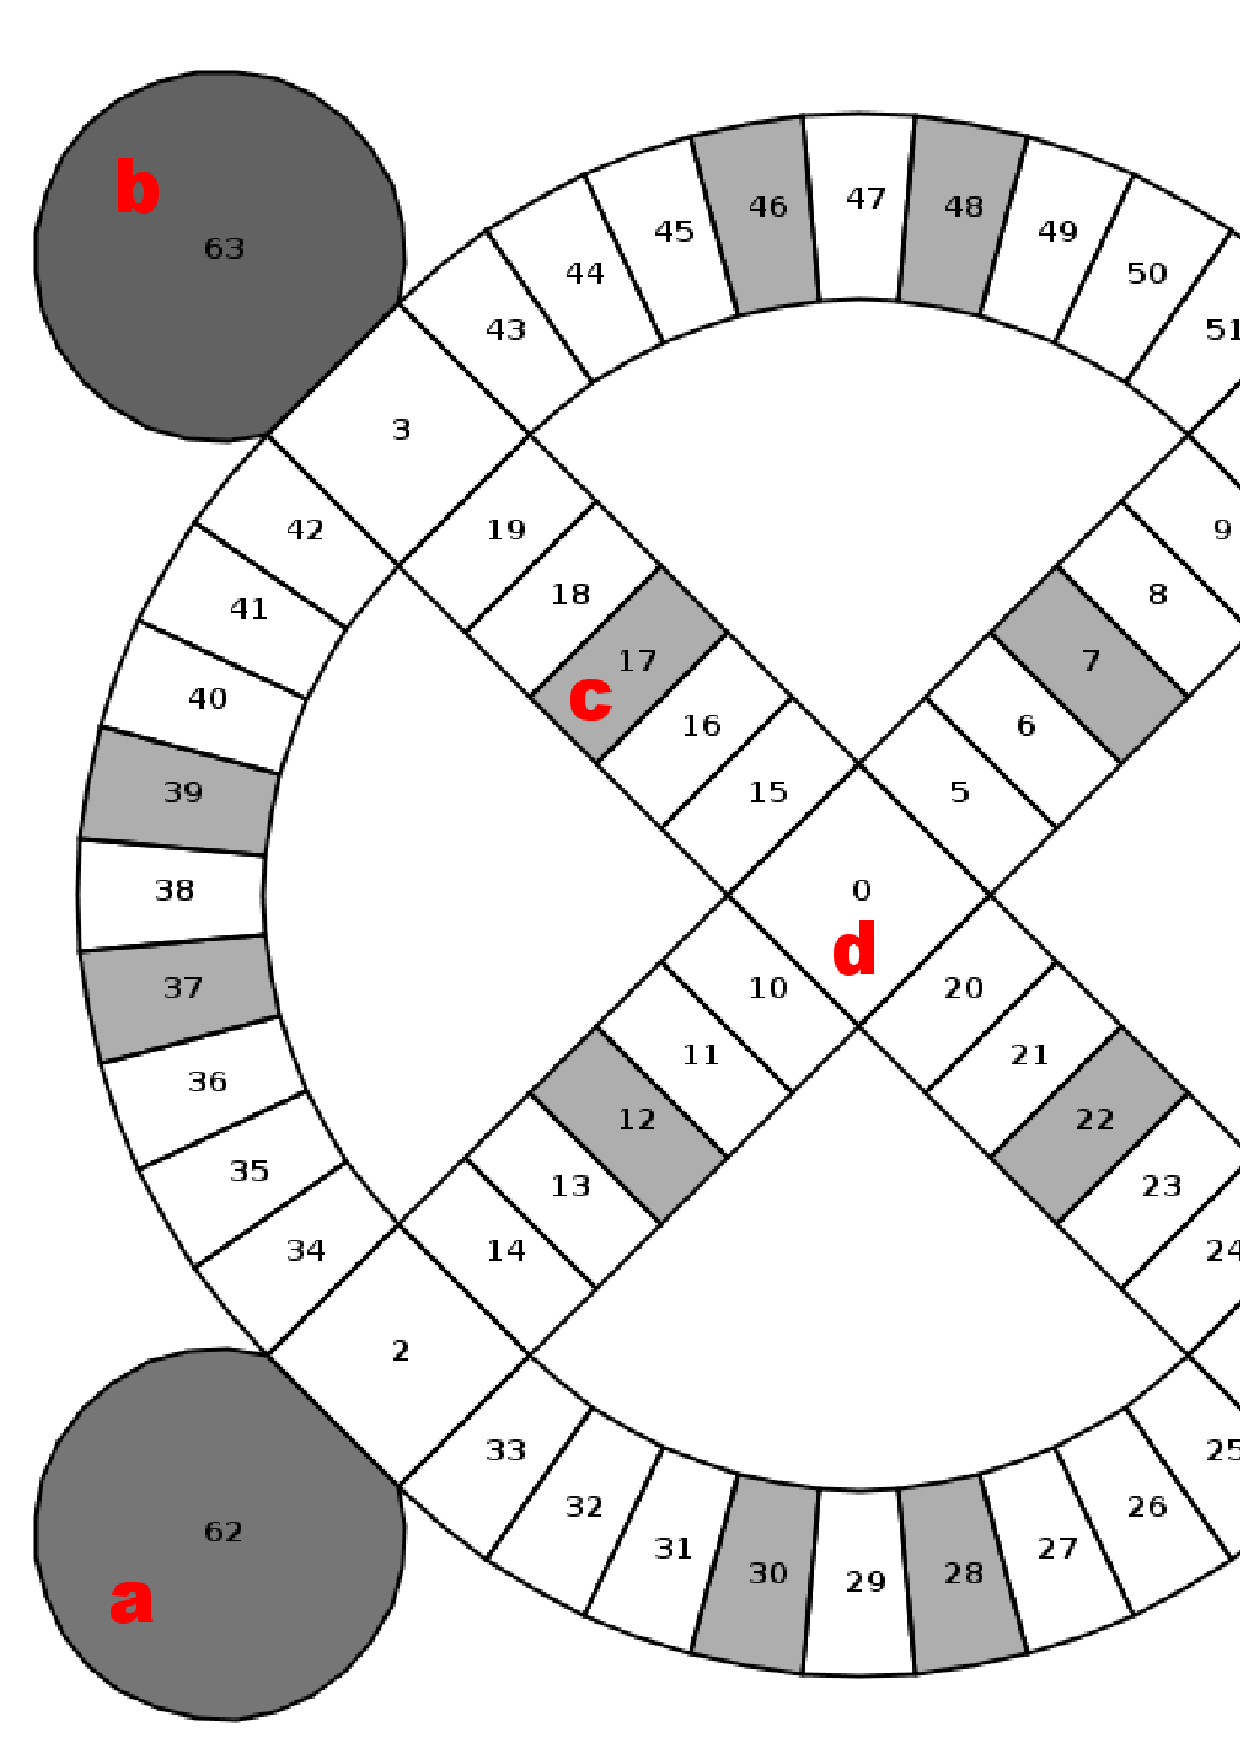
\includegraphics[scale=0.45]{ps/spielplan}}%
 \begin{pspicture}[showgrid=false](0,0)(\wd\SPIELPLAN,\ht\SPIELPLAN)
  \rput[lb](0,0){\usebox\SPIELPLAN}
  \rput( 1  , 1  ){\pscircle[fillstyle=solid,fillcolor=red,linestyle=none]{0.25}\rput[B](-.01,-.1){\white a}}
  \rput(11.75,11.75){\pscircle[fillstyle=solid,fillcolor=red,linestyle=none]{0.25}\rput[B](-.01,-.1){\white a}}

  \rput(11.75,1){\pscircle[fillstyle=solid,fillcolor=red,linestyle=none]{0.25}\rput[B](-.01,-.1){\white b}}
  \rput(1,11.75){\pscircle[fillstyle=solid,fillcolor=red,linestyle=none]{0.25}\rput[B](-.01,-.1){\white b}}

  \rput(4.3,7.75){\pscircle[fillstyle=solid,fillcolor=red,linestyle=none]{0.25}\rput[B](-.01,-.1){\white c}}

  \rput(6.3,5.95){\pscircle[fillstyle=solid,fillcolor=red,linestyle=none]{0.25}\rput[B](-.01,-.1){\white d}}
 \end{pspicture}
 \caption{Der Spielplan mit den Indizes der Spielfelder. Markiert sind a) die Heimatfelder des ersten Spielers, b) die Heimatfelder des zweiten Spielers, c) ein Sicherheitsfeld und d) ein normales Feld.}\label{spielplan}
\end{figure}

Auf einigen Feldern werden sich \textbf{Blumen} befinden. Die Schafe finden die Blumen sehr lecker und sollten so viele Blumen wie möglich sammeln und später fressen. Dies macht die Schafe glücklich und bringt dem Spieler Punkte.

Zusätzlich zu den Blumen befinden sich auf dem Spielplan auch \textbf{Fliegenpilze}.

Fliegenpilze verhalten sich genau wie Blumen. Sie werden also gesammelt, wenn ein Schaf ein entsprechendes Feld betritt und später gefressen. Allerdings gilt es, die Fliegenpilze zu vermeiden, denn sie bekommen den Schafen nicht gut und zählen daher \textbf{negativ}.

Abbildung \ref{blumen} zeigt, wie die Blumen und Fliegenpilze im Spiel aussehen.

\begin{figure}[!h]
 \centering
 \newsavebox\BLUMEN
 \sbox\BLUMEN{
\includegraphics[scale=0.6]{ps/blumen}}%
 \begin{pspicture}[showgrid=false](0,0)(\wd\BLUMEN,1.8)
  \rput[lb](0,0){\usebox\BLUMEN}
  \rput(0.5,1.5){\pscircle[fillstyle=solid,fillcolor=red,linestyle=none]{0.25}\rput[B](-.01,-.1){\white a}}
  \rput(2.225,1.5){\pscircle[fillstyle=solid,fillcolor=red,linestyle=none]{0.25}\rput[B](-.01,-.1){\white b}}
  \rput(4.0,1.5){\pscircle[fillstyle=solid,fillcolor=red,linestyle=none]{0.25}\rput[B](-.01,-.1){\white c}}
 \end{pspicture}
 \caption{Symbole für a) eine Blume, b) zwei Blumen und c) ein Fliegenpilz.}\label{blumen}
\end{figure}


\subsection{Spielfiguren}
Wie die Spielfelder hat auch jedes Schaf einen eindeutigen Index. Jedes Schaf ist genau einem der beiden Spieler zugeordnet. Im Spiel wird jedes Schaf durch eine Spielfigur in der Farbe seines Spielers dargestellt. Die Spielfiguren des Spielers, der nicht am Zug ist, werden grau dargestellt.

Ein Schaf kann im Laufe des Spiels gegnerische Schafe fangen bzw. in seine Herde aufnehmen. Hatte ein gegnerisches Schaf schon eigene Schafe gefangen, können so auch eigene Schafe in die Herde gelangen, sie werden also \textbf{zurückgefangen}. Wie bereits erwähnt, kann jedes Schaf Blumen oder Fliegenpilze sammeln. Daher befindet sich unterhalb jeder Spielfigur ein Statusbalken mit drei Zahlen, wie in Abbildung \ref{schafe} zu sehen ist.

\begin{figure}[!h]
 \centering
 \newsavebox\SCHAFE
 \sbox\SCHAFE{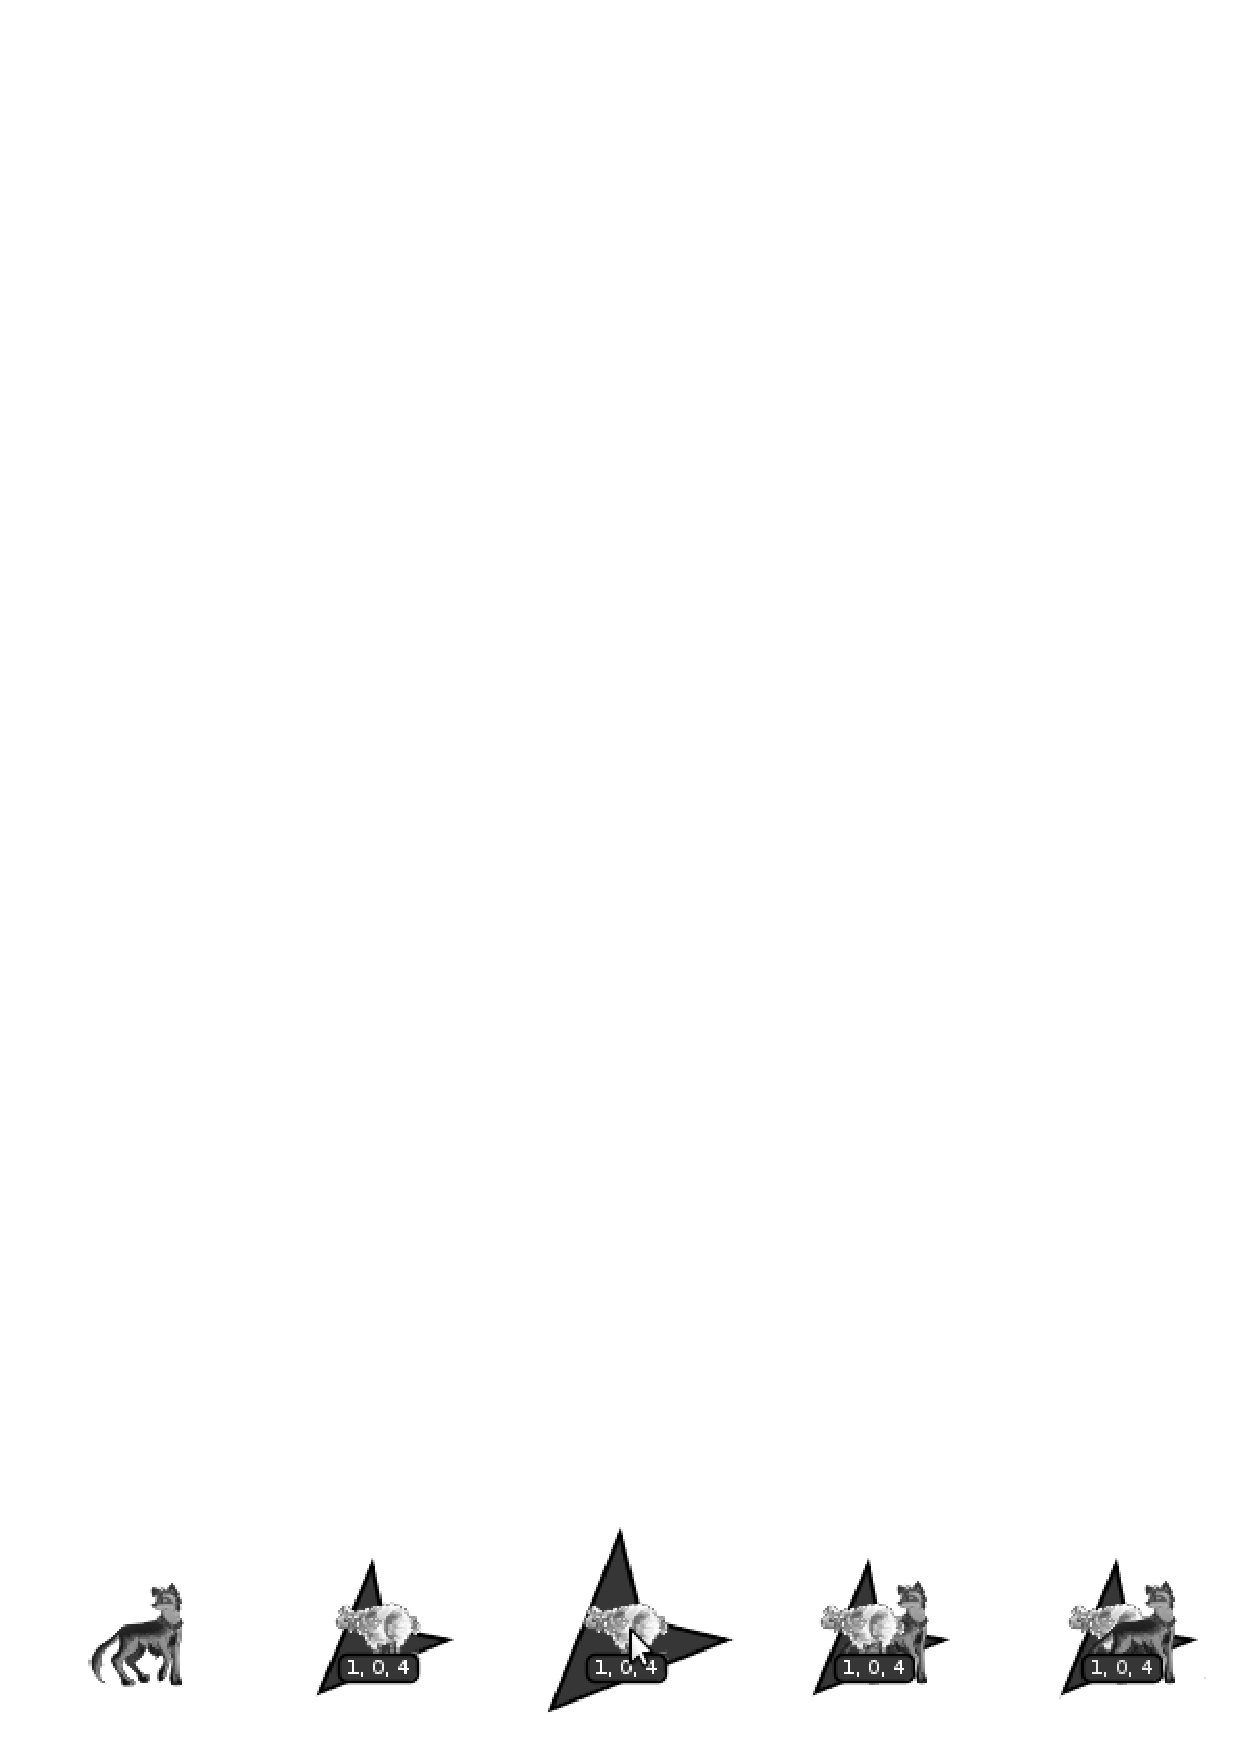
\includegraphics[scale=0.6]{ps/schafe}}%
 \begin{pspicture}[showgrid=false](0,0)(\wd\SCHAFE,2.1)
  \rput[lb](0,0){\usebox\SCHAFE}
  \rput(1.25,1.8){\pscircle[fillstyle=solid,fillcolor=red,linestyle=none]{0.25}\rput[B](-.01,-.1){\white a}}
  \rput(3.45,1.8){\pscircle[fillstyle=solid,fillcolor=red,linestyle=none]{0.25}\rput[B](-.01,-.1){\white b}}
  \rput(6,1.8){\pscircle[fillstyle=solid,fillcolor=red,linestyle=none]{0.25}\rput[B](-.01,-.1){\white c}}
  \rput(8.55,1.8){\pscircle[fillstyle=solid,fillcolor=red,linestyle=none]{0.25}\rput[B](-.01,-.1){\white d}}
  \rput(11.05,1.8){\pscircle[fillstyle=solid,fillcolor=red,linestyle=none]{0.25}\rput[B](-.01,-.1){\white e}}
 \end{pspicture}
 \caption{Die Spielfiguren für a) den Schäferhund zu Beginn, b) ein Schaf c), ein mit der Maus bewegtes Schaf, d) ein Schaf mit passivem Schäferhund und e) ein Schaf mit aktivem Schäferhund.}\label{schafe}
\end{figure}

\clearpage
Die drei Zahlne haben der Reihe nach die folgenden Bedeutungen:
\begin{itemize}
\item Die Anzahl der \textbf{eigenen Schafe} inklusive des Schafes, das durch diese Spilfigur symbolisiert wird. Diese Zahl kann daher nie unter 1 sinken.
\item Die Anzahl der gefangenen, \textbf{gegnerischen Schafe}. Diese Zahl kann nie unter 0 sinken.
\item Die Anzahl der gesammelten Blumen abzüglich der Anzahl der gesammelten Fliegenpilze. Diese Zahl kann also auch negativ werden.
\end{itemize}

Ein Schaf darf nach dem Verlassen eines Heimatfeldes nur das Heimatfeld betreten, das dem \textbf{von ihm zuletzt verlassenen} Heimatfeld \textbf{gegenüberliegt}. Ein Schaf darf also immer nur ein einziges Heimatfeld betreten. Unter der Spielfigur befindet sich ein Pfeil, der immer auf dieses Heimatfeld zeigt. Wird eine Spielfigur mit der Maus bewegt, wird der Pfeil etwas größer.

Zusätzlich zu den Schafen gibt es genau einen \textbf{Schäferhund}. Ein Schaf, das auf das Feld mit dem Schäferhund zieht, wird fortan von diesem \textbf{begleitet}. Wird ein von dem Schäferhund begleitetes Schaf von einem anderen Schaf gefangen, so begleitet der Schäferhund ab sofort das neue Schaf. Ist der Schäferhund also einmal mitgenommen worden, begleitet er von da an immer ein Schaf.

Zu Beginn des Spiels ist der Schäferhund \textbf{passiv}. Er wird \textbf{aktiv}, wenn er das erste Mal von einem Schaf mit \textbf{in ein Heimatfeld genommen} wird. Erst jetzt hat er einen Nutzen, denn er erlaubt es von da an dem von ihm begleiteten Schaf, auch gegnerische Schafe auf \textbf{Sicherheitsfeldern} zu fangen. Er beschützt ein Schaf aber \textbf{nicht} davor, selbst gefangen zu werden. Ist der Schäferhund einmal aktiv geworden, wird er nie wieder passiv.

\subsection{Würfel}
Im Spiel gibt es drei Würfel mit Augenzahlen zwischen 1 und 6. Eine Augenzahl gibt an, um wieviele Felder sich ein Schaf in einem Zug bewegen kann. Der Würfelvorrat wird von beiden Spielern gemeinsam benutzt und jedem Schaf steht jeder Würfel zur Verfügung. Es muss sich aber für eine der vorhandenen Augenzahlen entscheiden. 

Sobald ein Schaf eine Augenzahl genutzt hat, wird ein Würfel mit dieser Augenzahl neu gewürfelt. Der Wurf wird solange wiederholt, bis die folgenden beiden Bedingungen erfüllt sind:

\begin{itemize}
\item Den Schafen müssen zu jedem Zeitpunkt wenigstens zwei verschiedene Augenzahlen zur Verfügung stehen.
\item Der Spieler, der als nächstes am Zug ist, muss wenigstens einen gültigen Zug machen können.
\end{itemize}
 
\section{Spielaufbau}
Jeder Spieler beginnt mit \textbf{sechs} einzelnen Schafen. Je drei Schafe befinden sich in den beiden gegenüberliegenden Heimatfeldern. Der Schäferhund befindet sich zunächst in der Mitte des Spielplans auf dem Feld mit dem Index 0.

Zu Spielbeginn befindet sich je ein Fliegenpilz auf \textbf{acht} zufällig gewählten, normalen Feldern und \textbf{fünfzig} Blumen auf den übrigen normalen Feldern. Dabei bekommt jedoch kein Feld mehr als zwei Blumen. Es kann normale Felder geben, die weder Blumen noch Fliegenpilze haben.

Alle drei Würfel wurden unter Einhaltung der beiden zuvor genannten Bedingungen gewürfelt.

\section{Spielablauf}
Das Spiel ist rundenbasiert. In jeder Runde bewegt zunächst der erste Spieler eines seiner Schafe auf ein Feld, auf das dieses Schaf ziehen darf. Generell kann ein Schaf jedes Feld betreten, wenn der Abstand zwischen dem Feld, auf dem das Schaf steht, und dem Feld, auf das dieses Schaf ziehen will, der Augenzahl eines vorhandenen Würfels entspricht. Die Ausnahmen werden unten beschrieben. Danach wird ein Würfel mit der verwendeten Augenzahl den Regeln entsprechend neu gewürfelt. Anschließend macht auch der zweite Spieler einen solchen Zug und es wird erneut gewürfelt. Damit ist eine Runde beendet.

In den folgenden Fällen darf ein Schaf ein Spielfeld \textbf{nicht betreten}:

\begin{itemize}
\item Wenn es sich um ein gegnerisches Heimatfeld handelt.
\item Wenn es sich um das eigene Heimatfeld handelt, das von dem Schaf zuletzt verlassen wurde.

\item Wenn es sich um ein Sicherheitsfeld handelt, auf dem ein eigenes Schaf steht.
\item Wenn es sich um ein Sicherheitsfeld handelt, auf dem ein gegnerisches Schaf steht und das sich bewegende Schaf nicht in Begleitung des aktiven Schäfer\-hundes ist.

\item Wenn es sich um ein normales Feld handelt, auf dem bereits ein eigenes Schaf steht.
\end{itemize}

\subsection{Schafe bewegen}

Wird im Spiel eine Spielfigur mit der Maus bewegt, werden alle Felder, auf die das zugehörige Schaf ziehen darf, mit einem Rahmen \textbf{hervorgehoben}. Die Farbe des Rahmens entspricht der Farbe der Spielfigur. Auch eine Spielfigur des Spielers, der momentan nicht am Zug ist, kann mit der Maus bewegt werden. So kann man sich angucken, welche Felder ein Schaf theoretisch betreten könnte, wenn sein Spieler bereits am Zug wäre.

Zieht man eine Spielfigur des aktuellen Spielers über ein hervorgehobenes Spielfeld, so wird dieses Feld zusätzlich mit der Farbe der Spielfigur \textbf{hinterlegt}. Lässt man die Spielfigur über einem so hinterlegten Feld los, bewegt sich das Schaf auf dieses Feld.

Abbildung \ref{spielzug} zeigt, wie ein kompletter Spielzug im Spiel aussieht.

\begin{figure}[!h]
 \centering
 \newsavebox\SPIELZUG
 \sbox\SPIELZUG{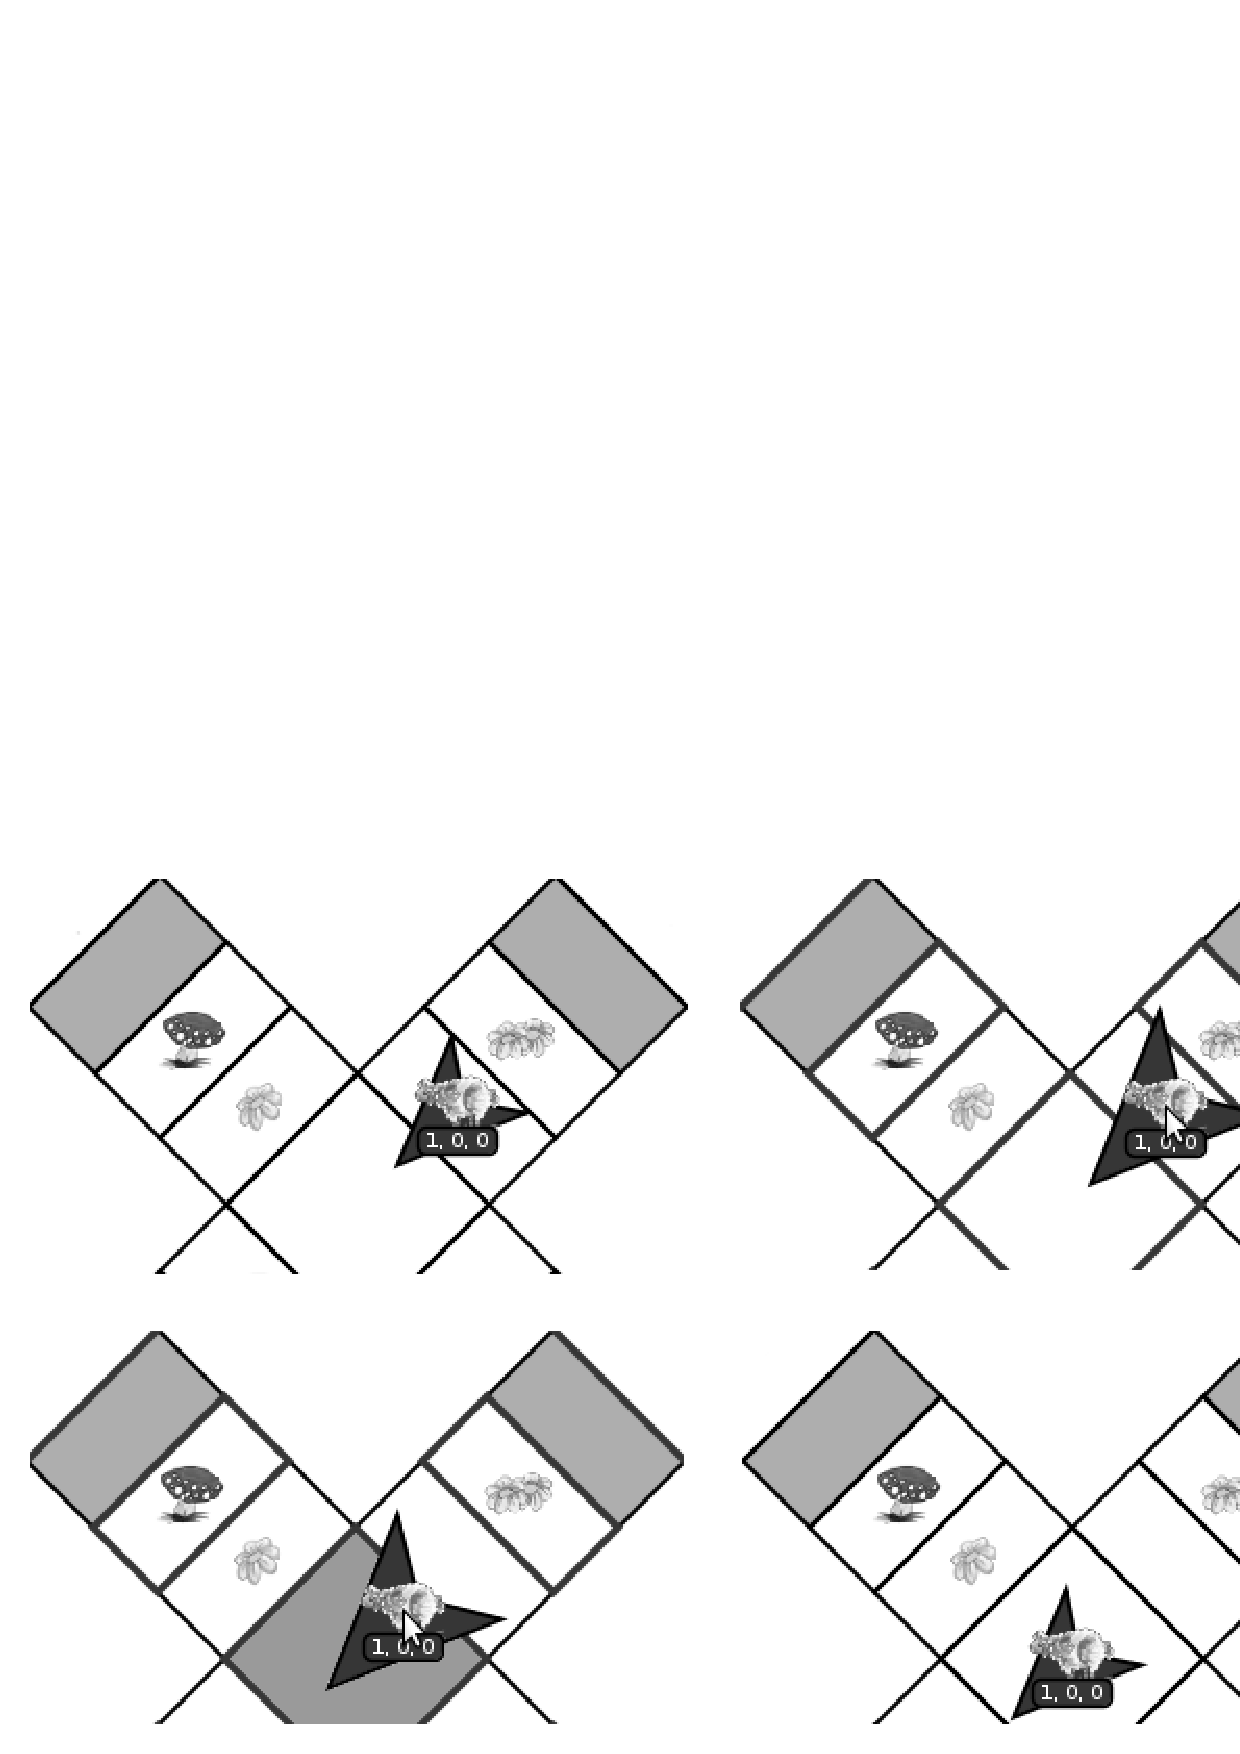
\includegraphics[scale=0.5]{ps/spielzug}}%
 \begin{pspicture}[showgrid=false](0,0)(\wd\SPIELZUG,\ht\SPIELZUG)
  \rput[lb](0,0){\usebox\SPIELZUG}
  \rput(2.755,6.05){\pscircle[fillstyle=solid,fillcolor=red,linestyle=none]{0.25}\rput[B](-.01,-.1){\white a}}
  \rput(8.85,6.05){\pscircle[fillstyle=solid,fillcolor=red,linestyle=none]{0.25}\rput[B](-.01,-.1){\white b}}
  \rput(2.755,2.2){\pscircle[fillstyle=solid,fillcolor=red,linestyle=none]{0.25}\rput[B](-.01,-.1){\white c}}
  \rput(8.85,2.2){\pscircle[fillstyle=solid,fillcolor=red,linestyle=none]{0.25}\rput[B](-.01,-.1){\white d}}
 \end{pspicture}
 \caption{Eine Spielfigur auf dem Spielplan a) vor dem Spielzug, b) mit hervorgehobenen Spielfeldern, c) mit hinterlegtem Spielfeld und d) nach dem Spielzug.}\label{spielzug}
\end{figure}

\subsection{Nach der Bewegung}
Bewegt sich ein Schaf auf ein Feld, so werden alle dort vorhandenen Blumen und Fliegenpilze eingesammelt.

Befindet sich ein gegnerisches Schaf auf dem Spielfeld, wird dieses Schaf gefangen. Alle von diesem nun gefangenen Schaf bereits gefangenen Schafe und eingesammelten Blumen und Fliegenpilze werden übernommen.

Wird ein Heimatfeld betreten, frisst das heimgekehrte Schaf alle von ihm gesammelten Blumen und Fliegenpilze. Sie sind endgültig aus dem Spiel raus. Alle mit nach Hause gebrachten Schafe werden aus dem Spiel entfernt\footnote{Die mitgebrachten, eigenen Schafe werden aus Implementierungsgründen nicht befreit. Er werden tatsächlich neue Schafe erstellt. Diese haben auch einen neuen, vorher nicht vergebenen Index.}. Dabei ist folgendes zu beachten:

\begin{itemize}
\item Handelte es sich um ein gegnerisches, also ein \textbf{gefangenes} Schaf, so ist es endgültig aus dem Spiel raus. Es ist nun \textbf{gestohlen}.
\item Handelte es sich um ein eigenes, also ein \textbf{zurückgefangenes} Schaf, so  wird in dieses Heimatfeld ein neues, eigenes Schaf gestellt.
\end{itemize} 

Nach einer Bewegung kann in einem Heimatfeld also niemals ein Schaf stehen, das von weiteren Schafen begleitet wird.

\section{Punkte}
Spielbegleitend werden Punkte nach den folgenden Regeln verteilt:

\begin{itemize}
\item Für jede gesammelte Blume gibt es zwei Punkte.
\item Für jeden gesammelten Fliegenpilz gibt es zwei Minuspunkte.
\item Für jede gefressene Blume gibt es zwei zusätzliche Punkte.
\item Für jeden gefressenen Fliegenpilz gibt es zwei zusätzliche Minuspunkte.
\item Für jedes gefangene, gegnerische Schaf gibt es acht Punkte.
\item Für jedes gestohlene, gegnerische Schaf gibt es acht zusätzliche Punkte.
\end{itemize}

\section{Spielende}
Das Spiel endet, sobald ein Spieler keine Schafe mehr hat; spätestens aber nach 30 gespielten Runden.

Ist das Spiel vorzeitig zu Ende, gewinnt der Spieler, der als einziger noch ein Schaf hat. Werden alle 30 Runden gespielt, gewinnt der Spieler mit mehr Punkten. Bei gleichem Punktestand ist das Spiel unentscheiden.

\section{Weitere Elemente}
Um das Spielfeld herum ist immer ein Rahmen in der Farbe des aktuellen Spielers gezeichnet.

An der rechten Seite befindet sich die in Abbildung \ref{seitenleiste} gezeigte Seitenleiste mit einigen Spielinformationen. Sie zeigt wie viele Blumen noch auf dem Spielfeld vorhanden sind. Von diesem Wert ist die Anzahl der noch vorhandenen Fliegenpilze bereits abgezogen, so dass zu Beginn des Spiels hier 42 steht. Darunter wird angezeigt, in der wievielten Runde sich das Spiel befindet.

In der normalen Ansicht werden darunter für beide Spieler einige Statusinformationen gezeigt. In der Debugansicht sind dieselben Informationen in einer kompakten Darstellung zu finden. 

\begin{figure}[!t]
 \centering
 \newsavebox\SEITENLEISTE
 \sbox\SEITENLEISTE{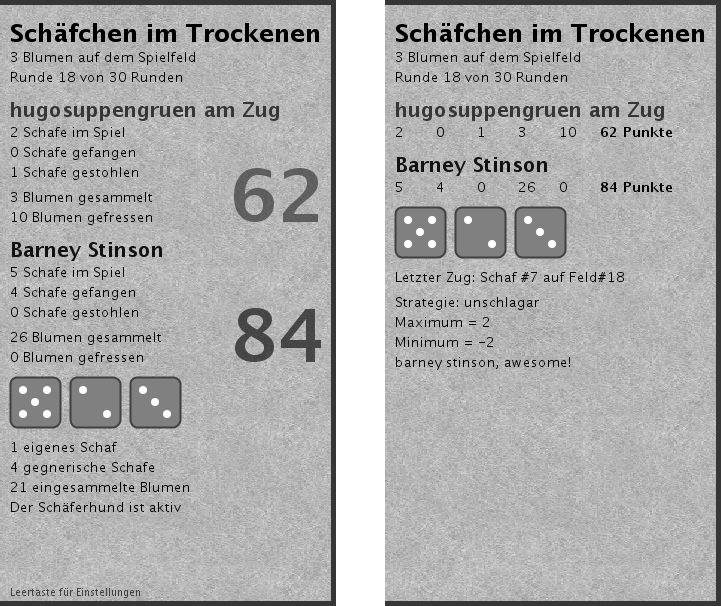
\includegraphics[scale=0.55]{ps/seitenleiste}}%
 \begin{pspicture}[showgrid=false](0,0)(\wd\SEITENLEISTE,\ht\SEITENLEISTE)
  \rput[lb](0,0){\usebox\SEITENLEISTE}
 
  \rput(3.2,11.75){\pscircle[fillstyle=solid,fillcolor=red,linestyle=none]{0.25}\rput[B](-.01,-.1){\white a}}
  \rput(10.7,11.75){\pscircle[fillstyle=solid,fillcolor=red,linestyle=none]{0.25}\rput[B](-.01,-.1){\white b}}

  \rput(-.1,10.5){\pscircle[fillstyle=solid,fillcolor=red,linestyle=none]{0.25}\rput[B](-.01,-.1){\white c}}
  \rput(7.4,10.5){\pscircle[fillstyle=solid,fillcolor=red,linestyle=none]{0.25}\rput[B](-.01,-.1){\white c}}

  \rput(3.5,6.9){\pscircle[fillstyle=solid,fillcolor=red,linestyle=none]{0.25}\rput[B](-.01,-.1){\white d}}
  \rput(11,8.55){\pscircle[fillstyle=solid,fillcolor=red,linestyle=none]{0.25}\rput[B](-.01,-.1){\white e}}

  \rput(4,35){\pscircle[fillstyle=solid,fillcolor=red,linestyle=none]{0.25}\rput[B](-.01,-.1){\white f}}
  \rput(11.45,7.25){\pscircle[fillstyle=solid,fillcolor=red,linestyle=none]{0.25}\rput[B](-.01,-.1){\white f}}

  \rput(3.33,2.7){\pscircle[fillstyle=solid,fillcolor=red,linestyle=none]{0.25}\rput[B](-.01,-.1){\white g}}

  \rput(7.4,6.35){\pscircle[fillstyle=solid,fillcolor=red,linestyle=none]{0.25}\rput[B](-.01,-.1){\white h}}

  \rput(10.1,5.35){\pscircle[fillstyle=solid,fillcolor=red,linestyle=none]{0.25}\rput[B](-.01,-.1){\white i}}

  \rput(3.05,.25){\pscircle[fillstyle=solid,fillcolor=red,linestyle=none]{0.25}\rput[B](-.01,-.1){\white j}}
 \end{pspicture}
 \caption{Die Seitenleiste in a) normaler Ansicht oder b) Debugansicht zeigt c) den aktuellen Spielstand, d) ausführliche Spielerinformation bzw. e) kompakte Spielerinformation, f) die vorhandenen Augenzahlen, g) Informationen über eine markierte Spielfigur, h) der letzte Spielzug, i) Debuginformationen und j) Hinweis auf das Einstellungsmenü.}\label{seitenleiste}
\end{figure}

Zudem werden die drei Würfel mit den momentan verfügbaren Augenzahlen angezeigt. 

Wird eine Spielfigur mit der Maus bewegt, werden in der normalen Ansicht nochmals die wichtigsten Informationen über diese Spielfigur angezeigt. In der Debugansicht werden die Kenndaten des letzten Zuges eingeblendet. Darunter befinden sich gegebenenfalls von einem Client gesendete Debuginformationen.

Hat das Spielfeld den Tastaturfokus, erscheint unten ein Hinweis auf das Einstellungsmenü. Um dem Spielfeld den Fokus zu geben, muss man ggf. einmal in das Spielfeld klicken. Hat das Spielfeld den Fokus, kann mit der \textbf{Leertaste} das in Abbildung \ref{einstellungen} gezeigte Menü geöffnet und wieder geschlossen werden. 

\begin{figure}[!t]
 \centering
 \newsavebox\EINSTELLUNGEN
 \sbox\EINSTELLUNGEN{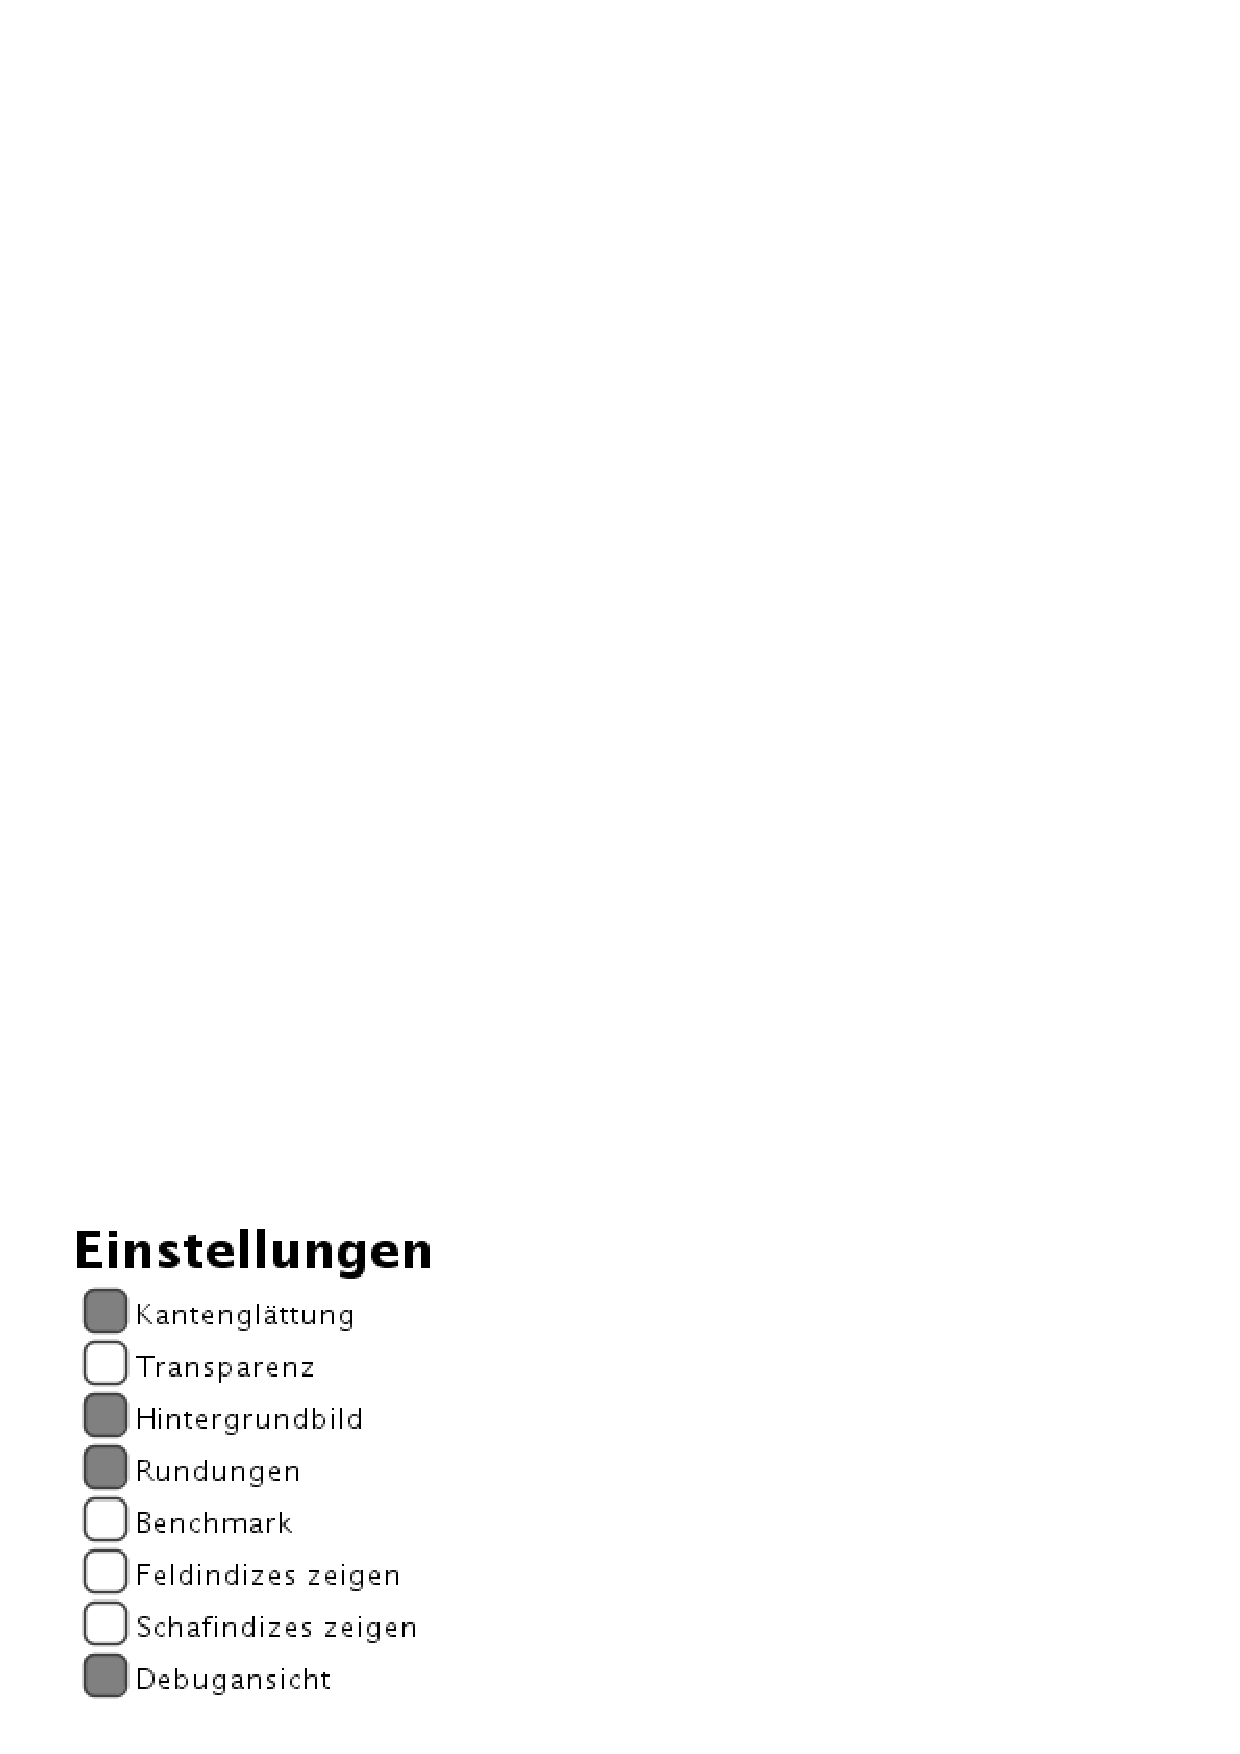
\includegraphics[scale=0.55]{ps/einstellungen}}%
 \begin{pspicture}[showgrid=false](0,0)(\wd\EINSTELLUNGEN,\ht\EINSTELLUNGEN)
  \rput[lb](0,0){\usebox\EINSTELLUNGEN}
 \end{pspicture}
 \caption{Das Einstellungsmenü.}\label{einstellungen}
\end{figure}


Die Optionen \textbf{Kantenglättung}, \textbf{Transparenz}, \textbf{Hintergrundbild} und \textbf{Rundungen} beeinflussen die grafische Darstellung des Spiels. Insbesondere die ersten beiden Optionen sind sehr rechenintensiv und sollten auf schwächeren Rechnern ausgeschaltet werden. Mit der Option \textbf{Benchmark} kann überprüft werden, ob die momentanen Einstellungen für den Rechner geeignet sind.

Über die Optionen \textbf{Feld--} und \textbf{Schafindizes zeigen} kann über jedem Feld bzw. Schaf der zugehörige, eindeutige Index eingeblendet werden.

Die Option \textbf{Debugansicht} legt fest, welche Seitenleiste angezeigt werden soll.


\end{document}


